\documentclass[12pt]{article}
\usepackage[a4paper, total={7.5in, 10.5in}]{geometry}
%\usepackage{array}
\usepackage{graphicx, subfig, wrapfig, fancyhdr, lastpage, multicol ,color,arydshln,makecell,chemfig}
\usepackage[most]{tcolorbox}
\newcommand\headerMe[2]{\noindent{}#1\hfill#2}
\usepackage[mathscr]{euscript}
\usepackage{tabularray}

\setlength{\columnseprule}{1pt}
\def\columnseprulecolor{\color{blue}}


\pagestyle{fancy}
\fancyhf{}

\cfoot{\vspace{-1cm} \em{Page \thepage \hspace{1pt} / 4}}


\newtcolorbox{Box2}[2][
enhanced, 
    breakable,
]{
                lower separated=false,
                colback=white,
colframe=white!20!black,fonttitle=\bfseries,
colbacktitle=white!30!gray,
coltitle=black,
enhanced,
attach boxed title to top left={yshift=-0.1in,xshift=0.15in},
title=#2,#1
}
%    \vspace{.2cm}



\begin{document}

\headerMe{Royaume du Maroc}{année scolaire \emph{2023-2024}}\\
\headerMe{Ministère de l'Éducation nationale, }{  }\\
\headerMe{du Préscolaire et des Sports}{Établissement : \emph{Lycée SKHOR qualifiant}}\\
\vspace{-1cm}
\begin{center}
	Devoir Surveillé  N°3 - S2 \\

	2ème année baccalauréat Sciences Mathématiques\\
	%Durée 2h00
	%    \vspace{.2cm}
	\hrulefill
  \Large{--Mécanique--}
	\hrulefill\\

	% \emph{Les  parties sont indépendantes}
	%\emph{Les deux parties sont indépendantes}

	\vspace{.2cm}
\end{center}
%end Headerss------------------------
%__________________Chimie ______________________-
%%%%%%%+_+_+_+_+_+_+_+_+_Partie1
\begin{Box2}{Etude énergétique d’un pendule pesant(2010SR)}


	\begin{wrapfigure}[10]{r}{0.2\textwidth}
		\begin{center}
			\vspace{-0.8cm}
			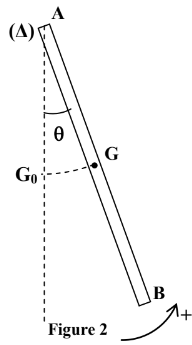
\includegraphics[width=0.2\textwidth]{./img/penduleP00.png}
		\end{center}
	\end{wrapfigure}

On considère un pendule pesant effectuant des oscillations libres non amorties .
Le pendule étudié est une tige AB homogène de masse m et
de longueur $AB = l = 60,0 cm$ pouvant tourner dans un plan
vertical autour d’un axe $\Delta$ horizontal passant par son extrémité A ,
figure (2).

  Le moment d’inertie de la tige par rapport à l’axe $\Delta$ est : $J_{\Delta} = \frac{1}{3}.ml^2$

On étudie le mouvement du pendule dans un repère lié au référentiel terrestre
que l’on suppose galileen .
On repère à chaque instant la position du pendule par l’abscisse angulaire $\theta$
qui est l’angle que fait la tige avec la verticale passant par A .
On choisit le plan horizontal passant par $G_0$ , position du centre d’inertie de
la tige AB dans la position d’équilibre stable , comme état de référence
pour l’ énergie potentielle de pesanteur( $E_p = 0$) .

  On admet dans le cas de faibles oscillations que $cos\theta \approx 1 - \frac{\theta^2}{2}$
et on prend 

  $g = 9,80 m.s^{-2}$

  \textbf{1- Equation différentielle du mouvement du pendule}

  \begin{enumerate}
    \item Montrer que l’expression de l’énergie potentielle de pesanteur Ep de la tige peut s’écrire sous la
      forme $E_p = m.g.\frac{l}{2}(1 - cos(\theta))$.
    \item Dans le cas de faibles oscillations , écrire l’expression de l’énergie mécanique $E_m$ de la tige à un
instant t en fonction de $m$ , $l$ , $g$ , $\theta$ et $\frac{d\theta}{dt}$
\item Déduire l’équation différentielle vérifiée par l’abscisse angulaire dans le cas de faibles oscillations.
  \end{enumerate}

  \textbf{2- Etude énergétique}

	\begin{wrapfigure}[10]{r}{0.4\textwidth}
		\begin{center}
			\vspace{-2cm}
			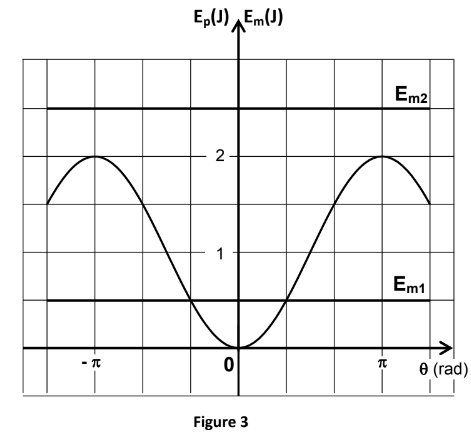
\includegraphics[width=0.4\textwidth]{./img/PenduleP01.png}
		\end{center}
	\end{wrapfigure}

  On lance la tige AB à partir de sa position d’équilibre stable avec une vitesse initiale qui lui permet
d’acquérir une énergie mécanique $E_m$ .
La figure 3 donne le diagramme de l’évolution de l’énergie potentielle $E_p$ et de l’énergie mécanique $E_m$
de la tige AB pour deux expériences différentes .Dans chaque expérience la tige est lancée à partir de sa
position d’équilibre stable avec une vitesse initiale donnée ; elle acquiert dans chaque expérience une
énergie mécanique donnée :

  - dans l’expérience (1) : $E_m=E_{m1}$

  - dans l’expérience (2) : $E_m=E_{m2}$

\begin{enumerate}
    \item Déterminer à l’aide du graphe,
de la figure (3), la nature du mouvement
de la tige dans chaque expérience .

  \item Préciser à partir du graphe la valeur
maximale de l’abscisse angulaire $\theta$
du pendule dans l’expérience (1).
En déduire la masse m de la tige.
  
  \item Au cours de l’expérience (2) , l’énergie
cinétique de la tige varie entre une valeur
      minimale $E_{c(min)}$ et une valeur
      maximale $E_{c(max)}$.Trouver la valeur de Ec(min) et celle de Ec(max)
\end{enumerate}

\end{Box2}

\begin{Box2}{Changement des conditions initiales du mouvement d’un oscillateur
  non amorti(2010SN)}

	\begin{wrapfigure}[14]{r}{0.4\textwidth}
		\begin{center}
			\vspace{-0.6cm}
			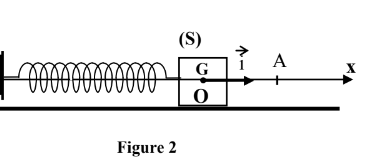
\includegraphics[width=0.4\textwidth]{./img/penduleE.png}
			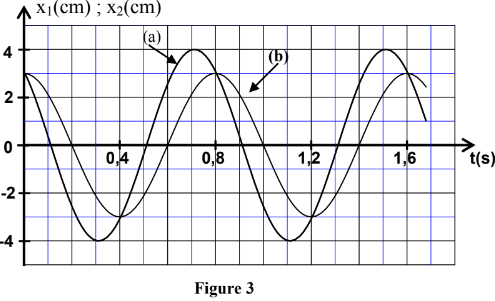
\includegraphics[width=0.4\textwidth]{./img/penduleE01.png}
		\end{center}
	\end{wrapfigure}


Un système mécanique oscillant est un système qui effectue un mouvement périodique de
va et vient autour de sa position d’équilibre stable.

Un pendule élastique horizontal est constitué d’un solide (S) de masse m lié à l’extrémité d’un
ressort à spires non jointives , de masse négligeable de raideur K . L’autre extrémité du ressort est
liée à un support fixe ,figure (2).

A l’équilibre , le centre d’inertie G du solide(S)
  coïncide avec l’origine O du repère d’espace $(O,\vec{i})$ lié à la Terre .

  On écarte le solide (S) de sa position d’équilibre dans
le sens positif jusqu’à ce que son centre d’inertie G
coïncide avec un point A situé à une distance d du point O .
On considère les deux cas suivants :

- 1er cas : On abandonne à t = 0 le corps (S) au point A sans vitesse initiale .

- 2ème cas : On lance à t = 0 , le corps (S) à partir du point A dans le sens négatif avec une
vitesse initiale $\vec{v_A}$.

Dans les deux cas le solide (S) effectue un mouvement oscillatoire autour de sa position
d’équilibre O .

\begin{enumerate}
  \item Etablir l’équation différentielle que vérifie l’abscisse x du centre d’inertie G du solide .
  \item Trouver l’expression littérale de la période propre T0 de l’oscillateur pour que l’équation
    $x(t) = X_m.cos(\frac{2.\pi}{T_0}.t + \phi)$ soit solution de l’équation différentielle.
  \item On obtient à l’aide d’un dispositif approprié la courbe d’évolution des abscisses $x_1$ et $x_2$ du
centre d’inertie G du corps (S) successivement dans le 1er et le 2ème cas comme l’indique
la figure (3) .
Préciser , en justifiant la réponse , la courbe correspondante au mouvement de l’oscillateur dans
le 1er cas .
\item On considère l’oscillateur dans
le 2ème cas et on désigne l’amplitude
    de son mouvement par $x_{m2}$ et la phase
à l’origine des dates par $\phi_2$.
\begin{enumerate}
  \item Déterminer à partir du graphe,
figure (3) la valeur de la distance d
    et la valeur de l’amplitude $x_{m2}$ .
  \item En appliquant la conservation de
l’énergie mécanique , montrer que
    l’amplitude $x_{m2}$ peut s’écrire sous
    la forme : $$X_{m2} = \sqrt{\frac{m.v_A^2}{K} + d^2}$$
  \item Trouver l’expression de $tan(\phi_2)$ en fonction de d et $x_{m2}$ .
\end{enumerate}
\end{enumerate}

\end{Box2}

\begin{Box2}{Mesure de la masse d’un corps à l’intérieur d’une navette spatiale en
  orbite(2008SR) }

	\begin{wrapfigure}[10]{r}{0.4\textwidth}
		\begin{center}
			\vspace{-0.6cm}
			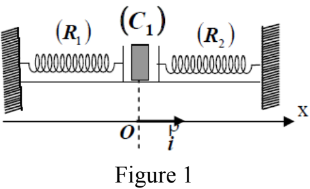
\includegraphics[width=0.34\textwidth]{./img/double_pendule00.png}
      
		\end{center}
	\end{wrapfigure}


  \emph{Lors des recherches à l’intérieur d’une navette spatiale en orbite autour de la Terre,
un astronaute mesure les masses de quelques corps en utilisant un dispositif
constitué d’un compartiment (A) de masse m = 200 g, susceptible de glisser sans
frottements sur un plan horizontal. Le compartiment est relié aux extrémités de
deux ressorts (R1) et (R2) de même raideur K et de même longueur à vide l0, et dont
les autres extrémités sont fixées à deux supports fixes.
A l’équilibre, les deux ressorts sont allongés.}
 
	Avant l’utilisation du dispositif en orbite, il a été testé sur Terre.
Un corps ($C_1$) de masse $M = 100 g$, est posé à
l’intérieur du compartiment (A).

Le système (S) formé du compartiment (A) et
du corps ($C_1$) est écarté de sa position
d’équilibre $G_0$ coïncidant avec l’origine de l’axe
(O,i)
, vers la droite d’une distance $X_m$ et lâché
sans vitesse initiale.
\begin{wrapfigure}[14]{r}{0.4\textwidth}
		\begin{center}
			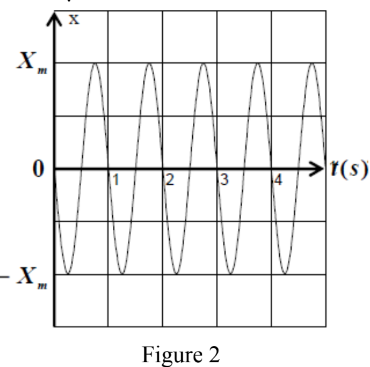
\includegraphics[width=0.4\textwidth]{./img/double_Pendule.png}
		\end{center}
	\end{wrapfigure}



Le centre de gravité G du système (S), effectue des oscillations autour de sa position
d’équilibre de telle sorte que les ressorts restent allongés.
Un ordinateur muni d’une carte d’acquisition, permet d’obtenir la courbe
représentative des variation de l’abscisse x du centre de gravité G au cour du temps
(Figure 2).
\begin{enumerate}
  \item Montrer que les deux ressorts ont la même longueur initiale à l’équilibre : $\Delta{l_1}  = \Delta{l_2} = \Delta{l_0}$
  \item Montrer que l’abscisse x du centre de gravité G du système (S) vérifie
    l’équation différentielle : $$\ddot{x} + \frac{2K}{m + M_1}x = 0$$
  \item La solution de cette équation
    différentielle s’écrit sous la forme : $x(t) = X_m.cos(\frac{2.\pi.t}{T_0} + \phi)$.
    \begin{enumerate}
      \item Trouver à partir de la courbe,
la phase $\phi$ du mouvement.
\item En utilisant l’équation
différentielle et sa solution,
trouver l’expression de la
période propre $T_0$ du
mouvement en fonction de :
$M_1$, m et $K$.
\item Par exploitation du graphe de la figure 2, calculer la valeur de la raideur K
du ressort.


On prendra $\pi^2= 10$.
\item L’astronaute réalise la même expérience, en utilisant le même corps ($C_1$)
et le même dispositif, dans une navette spatiale en orbite autour de la
terre, il trouve la même valeur de la période $T_0$. Que conclure ?
\item L’astronaute utilise le même dispositif précédent pour mesurer la masse
$M_2$ d’un corps ($C_2$) en orbite, il trouve que la période propre des
oscillations du système est $T’0$=$1,5s$. En déduire la valeur de M2.
    \end{enumerate}
    
\end{enumerate}

\end{Box2}

\begin{Box2}{mouvement d’un sportif sur un plan incliné (2009 SR) }

	\begin{wrapfigure}[9]{r}{0.4\textwidth}
		\begin{center}
			\vspace{-0.6cm}
			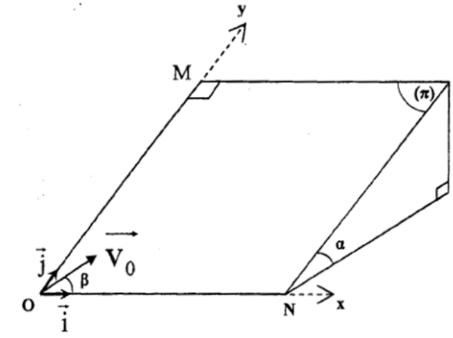
\includegraphics[width=0.34\textwidth]{./img/incl00.png}
      
		\end{center}
	\end{wrapfigure}
  Un sportif de masse $m = 60 kg$, glisse sur un plan $(\pi)$ incliné d’un angle $\alpha = 12^{\circ}$
par rapport au plan horizontal.
Le plan $(\pi)$ a la forme d’un rectangle de longueur OM et de largueur $ON = 20 m$
(Figure 1).

On modélise le sportif par un solide (S) de masse m et de centre d’inertie G.
On étudie le mouvement de G dans le repère orthonormé
$(O, \vec{i}, \vec{j})$ : où $(O,\vec{i})$ est  horizontal, et
  $(O, \vec{j})$

  parallèle à la ligne de plus grande pente du plan ($\pi$).

On néglige tous les frottements.
  On prendra :$ g = 9,80 m.s^{-2}$

  \textbf{1- Etude d’un mouvement plan sur un plan incliné :}
  A l’instant t = 0, le centre d’inertie G du sportif passe en O origine du repère
$(O, \vec{i}, \vec{j})$ avec une vitesse de vecteur $\vec{v_0}$ , contenu dans le plan ($\pi$), et faisant un angle $\beta$ avec l’axe $(O,\vec{i})$.

\begin{enumerate}
  \item Montrer que les composantes du vecteur vitesse, à un instant t, vérifient les
    équations différentielles : $\frac{dV_x}{dt} = 0$ et $\frac{dV_y}{dt} = -g.sin\alpha$
  \item Trouver l’équation de la trajectoire de G dans le repère $(o, \vec{i}, \vec{j})$
  \item Dans le cas où $\beta = 60^{\circ}$ :

    \begin{enumerate}
      \item Calculer la valeur de $v_0$ pour que G passe au point N.
      \item Trouver les expressions des coordonnées $x_S$ et $y_S$, du point S, sommet
de la trajectoire de G, en fonction de $v_0$, $\alpha$, $\beta$ et g.
    \end{enumerate}
\end{enumerate}
  \textbf{2 - Etude d’un mouvement oscillatoire sur un plan incliné :}

		\begin{center}
			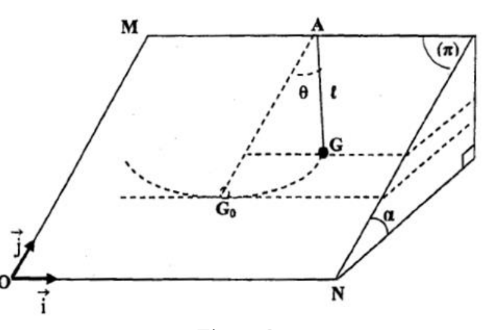
\includegraphics[width=0.34\textwidth]{./img/incli01.png}
      
		\end{center}


  Le sportif tient le bout d’une corde dont l’autre extrémité est fixée au point A se
trouvant au haut du plan incliné $(\pi)$. Il commence à effectuer des petites oscillations
autour de sa position d’équilibre $AG_0$ parallèle à l’axe
  $(O, \vec{j})$ .

Pour étudier le mouvement du sportif tenant la corde, on le modélise par un pendule
simple, constitué d’un solide de masse m et de centre d’inertie G, accroché à un fil
inextensible, de masse négligeable, parallèle au plan $(\pi)$ et de longueur l = 12 m
(Figure 2)

On repère, à chaque instant, la position de G par l’abscisse angulaire $\theta$ formé entre la
corde et la droite ($AG_0$).

On prendra comme état de références de l’énergie potentielle de pesanteur $(Epp = 0)$,
le plan horizontal passant par $G_0$.

Le moment d’inertie $J_\Delta$ par rapport à l’axe de rotation ($\Delta$) passant par A est : $J_{\Delta} = ml^2$

\begin{enumerate}
  \item Montrer que l’énergie mécanique du pendule s’écrit $$\frac{1}{2}.ml^2.[\frac{g.sin\alpha}{l}.\theta^2 + (\frac{d\theta}{dT})^2]$$
  \item En déduire l’équation différentielle vérifiée par l’abscisse angulaire.
  \item Trouver, par utilisation de l’équation différentielle et de sa solution,
l’expression de $T_0$. Calculer sa valeur.
\item Calculer, au passage du centre d’inertie G par $G_0$, l’intensité de la tension $\vec{T}$ appliquée par la corde sur le solide, dans le cas où $\theta_m = 12^{\circ}$.
\end{enumerate}
\end{Box2}



\end{document}
